\documentclass{article}
\usepackage{amsmath}
\usepackage{tikz}
\usepackage{fancybox}

\title{Analysis of Algorithms Final}
\author{Jay R Bolton}

\addtolength{\oddsidemargin}{-.875in}
\addtolength{\evensidemargin}{-.875in}
\addtolength{\textwidth}{1.75in}
\addtolength{\topmargin}{-.875in}
\addtolength{\textheight}{1.75in}

\begin{document}
\maketitle

\begin{enumerate}
\setlength{\leftmargin}{0pt}

\item[\textbf{1}]

	\begin{enumerate}
	 
	\item[\textbf{\emph{(a)}}]

$height = log_3n$

\ovalbox{
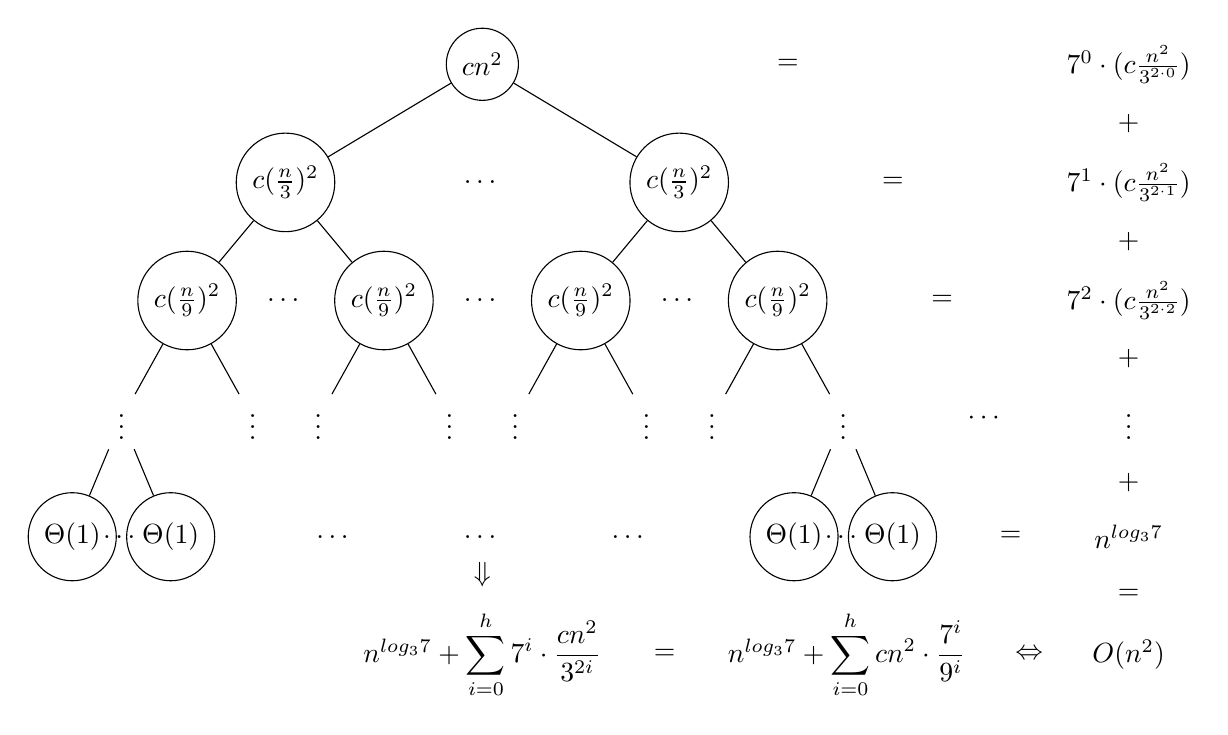
\begin{tikzpicture}[level/.style={sibling distance=50mm/#1}]
\node [circle,draw] (z){$cn^2$}
	child {node [circle,draw] (a) {$c(\frac{n}{3})^2$}
    child {node [circle,draw] (b) {$c(\frac{n}{9})^2$}
      child {node {$\vdots$}
				child {node [circle,draw] (d) {$\Theta(1)$}}
				child {node [circle,draw] (e) {$\Theta(1)$}}
      } 
      child {node {$\vdots$}}
    }
    child {node [circle,draw] (g) {$c(\frac{n}{9})^2$}
      child {node {$\vdots$}}
      child {node {$\vdots$}}
    }
  }
  child {node [circle,draw] (j) {$c(\frac{n}{3})^2$}
    child {node [circle,draw] (k) {$c(\frac{n}{9})^2$}
      child {node {$\vdots$}}
      child {node {$\vdots$}}
    }
  child {node [circle,draw] (l) {$c(\frac{n}{9})^2$}
    child {node {$\vdots$}}
    child {node (c){$\vdots$}
			child {node [circle,draw] (o) {$\Theta(1)$}}
			child {node [circle,draw] (p) {$\Theta(1)$}
        child [grow=right] {node (q) {$=$} edge from parent[draw=none]
					child [grow=right] {node (q) {$n^{log_37}$} edge from parent[draw=none]
            child [grow=up] {node (r) {$\vdots$} edge from parent[draw=none]
              child [grow=up] {node (s) {$7^2 \cdot (c\frac{n^2}{3^{2\cdot 2}})$} edge from parent[draw=none]
                child [grow=up] {node (t) {$7^1 \cdot (c\frac{n^2}{3^{2\cdot 1}})$} edge from parent[draw=none]
									child [grow=up] {node (u) {$7^0 \cdot (c\frac{n^2}{3^{2\cdot 0}})$} edge from parent[draw=none]}
                }
              }
            }
            child [grow=down] {node (v) {$O(n^2)$}edge from parent[draw=none]}
          }
        }
      }
    }
  }
	%child {node [grow=left] (aa) {$h= log_3 n$}edge from parent[draw=none]}
};
\path (a) -- (j) node [midway] {\dots};
\path (b) -- (g) node [midway] {\dots};
\path (k) -- (l) node [midway] {\dots};
\path (k) -- (g) node [midway] {\dots};
\path (d) -- (e) node [midway] {\dots};
\path (o) -- (p) node [midway] {\dots};
\path (o) -- (e) node (x) [midway] {$\dots$}
  child [grow=down] {
		node (y) {$n^{log_37} + \displaystyle\sum_{i = 0}^h 7^i \cdot \frac{cn^2}{3^{2i}}$}
    edge from parent[draw=none]
  };
\path (q) -- (r) node [midway] {+};
\path (s) -- (r) node [midway] {+};
\path (s) -- (t) node [midway] {+};
\path (s) -- (l) node [midway] {=};
\path (t) -- (u) node [midway] {+};
\path (z) -- (u) node [midway] {=};
\path (j) -- (t) node [midway] {=};
\path (y) -- (x) node [midway] {$\Downarrow$};
\path (v) -- (y)
node (w) [midway] {$n^{log_37} + \displaystyle\sum_{i = 0}^h cn^2 \cdot \frac{7^i}{9^i}$};
\path (q) -- (v) node [midway] {=};
\path (e) -- (x) node [midway] {\dots};
\path (o) -- (x) node [midway] {\dots};
\path (y) -- (w) node [midway] {$=$};
\path (v) -- (w) node [midway] {$\Leftrightarrow$};
\path (r) -- (c) node [midway] {$\cdots$};
\end{tikzpicture}}

		\item[\textbf{\emph{(b)}}]
			\begin{align*}
				& \sum_{i=0}^{log_3n} \frac{7^icn^2}{3^{i2}} + n^{log_37} \\
				<&\ cn^2 \sum_{i=0}^{\infty} \frac{7^i}{9^{i}} + n^{log_37} \\
				=&\ cn^2 \frac{1}{1 - 7/9} + n^{log_37} \\
				=&\ 3cn^2 + n^{log_37} \\
				<&\ 4cn^2 \\
				=&\ \mathcal{O}(n^2)
			\end{align*}

		\item[\textbf{\emph{(c)}}]

			Induction for $\mathcal{O}$

			\begin{align*}
			& \text{Inductive Hypothesis: } T(n) \geq cn^2\\
			& \text{Induction: } T(n) \geq 7c\frac{n^2}{3^2} + dn^2 \\
			& = cn^2 \frac{7}{9} + dn^2 \\
			& \geq cn^2 \ \ \ \ \text{with $c \leq 4d$ and $n \geq 0$}
			\end{align*}

			Induction for $\Omega$

			\begin{align*}
			& \text{Inductive Hypothesis: } T(n) \leq cn^2\\
			& \text{Induction: } T(n) \leq 7c\frac{n^2}{3^2} + dn^2 \\
			& = cn^2 \frac{7}{9} + dn^2 \\
			& \leq cn^2 \ \ \ \ \text{with $c \geq 5d$ and $n \geq 0$}
			\end{align*}

		\item[\textbf{\emph{(d)}}]

			\begin{align*}
			& a = 7,\ b = 3 \\
			& f(n) = n^2 = \Omega(n^{log_37 + \epsilon}) \\
			& lim_{n\rightarrow \infty}\frac{n^2}{n^{log_37+ \epsilon}} < \infty \text{   (it is polynomially larger)} \\
			& \text{Regularity condition:} \\
			& 7\frac{n^2}{3^2} \leq cn^2 \\ 
			& = \frac{7}{9}n^2 \leq cn^2 \ \ \ \ \text{ for $c \geq 7/9$ and $c \leq 1$ and $n \geq 0$}\\ 
			& \text{(Passes)} \\
			& \text{Case 3: } \Theta(n^2)
			\end{align*}

	\end{enumerate}

	\item[\textbf{2}]
	
		\begin{enumerate}
		\item[\textbf{\emph{(a)}}]
			
			I'll use the four conditions listed in our book on page 379. It took me a
			bit to realize how this was not a greedy choice problem. Tricky!

			\begin{enumerate}
			\item Our inital choice can be a division that we make of $C$, where
			$C_{choice} < C$ is optimal and $C-C_{choice}$ is our subproblem.
			\item The optimal choice given to us would be the sum $C_{choice}$, which
			is less than $C$ so divides it at some point.
			\item The subproblem that ensues is $C- C_{choice}$ which is the
			remaining sum we have yet to find an optimum on.
			\item Suppose we have come to an optimal solution with suboptimal
			$C_{choice}$ and $C-C_{choice}$. If we ``cut'' away our two suboptimal
			subproblems and replace them with more optimal ones, then we would
			supposedly increase the optimality of the whole problem. But this is a
			contradiction of our suppostion that we had an optimal solution.
			\end{enumerate}

		\item[\textbf{\emph{(b)}}]

			In haskell:

\begin{verbatim}
vs = [1,5,10,25,100,200]

change 0 _ = 0
change c [1] = c
change c v
 | last v <= c = min (change c (init v)) (1 + change (c-(last v)) v)
 | last v > c  = change c (init v)

-- >> change 7 vs
-- >> 3
-- >> change 42 vs
-- >> 5
\end{verbatim}

			With memoization:

\begin{verbatim}
-- Generate our memoization matrix.
-- There's probably a prettier way to do it, perhaps with list comp.
matrix c v = map (\(n,cs) -> (map (\c -> (n,c)) cs)) (zip [1..n] (replicate n [c,c-1..1]))
 where n = length v
-- Map our change function over the matrix
change_matrix c v = map (map (\(x,y) -> ch y (take x v))) (matrix c v)
 where
 ch 0 _ = 0
 ch c [1] = c
 ch c v
  | last v <= c = min (mchange c (init v)) (1 + mchange (c-(last v)) v)
  | last v > c  = mchange c (init v)
  where n = length v

-- Get the cell in the matrix for which we used n coins on c sum
mchange c v = (change_matrix c v) !! (length v - 1) !! 0

-- >> mchange 7 vs
-- >> 3
-- >> mchange 42 vs
-- >> 5
\end{verbatim}

			That was fun. It seems to work correctly but I'm not entirely sure it
			memoizes rather than recomputes the matrix every time. I've read before
			about using a fixed point function to factor out memoization in haskell
			that looked really neat but I probably don't have time to figure it out.

		\item[\textbf{\emph{(c)}}]

			For each coin $v(n)$ we have to consider $min(f(C-v(n),n), f(C-v(n-1),n),
			\dots, f(C-v(1),n))$ where f is our choice function. That amounts to $n$
			total choices per coin.

		\item[\textbf{\emph{(d)}}]
			
			Since for each coin we must consider $n$ subproblems, and the worst case
			is $C$ total coins, our complexity would then be $\Theta(Cn)$ total
			choices overall.

			Here is a greedy version of the algorithm I made before realizing it
			isn't optimal. Might as well leave it here.

			\begin{align*}
			& \text{Let $C$ be our goal sum and $v(n)$ be the coin of $n^{th}$ value.} \\
			& NCoins(C,1) = C \\
			& NCoins(C,n) = NCoins(C\ \%\ v(n), n-1) + \lfloor C/v(n) \rfloor
			\end{align*}

		\end{enumerate}

		\item[\textbf{3}]

		\begin{enumerate}

			\item[\textbf{\emph{(a)}}]

			I'll use the conditions on page 423 of our book:

				\begin{enumerate}
					\item 
						Suppose there are two leaves, $x$ and $y$, having both the least
						weights and the largest depths. To show that this is a greedy
						choice problem, we can show that the tree with $x$ and $y$ as
						given is an optimal tree (labeled $T$).

						By contradiction let's suppose that these two leaves with the two
						largest depths are not $x$ and $y$ so do not have the least
						weights. Instead they are $b$ and $d$ which produces the supposed
						optimal $T'$.

						Now let's swap one of the least weights, $x$, with one of the
						lowest leaves, $b$, to get a new tree $T''$. Let $d(b) - d(x)$ from
						$T'$ be $diff$. The depth of $x$ in $T''$ is increased by $diff$
						while the depth of $b$ is decreased by $diff$.

						The cost of our new tree is then: $cost(T'') = cost(T') +
						diff(cost(x) - cost(b))$. By supposition however, $cost(x) \leq
						cost(b)$, so $diff(cost(x) - cost(b)) \leq 0$. That means by
						swapping $x$ and $b$ to put $x$ in one of the two lowest leaves, we
						get $T''$ which is more optimal than $T'$. This is more optimal so
						contradicts our supposition. We can do the same procedure on $y$
						and $d$.

					\item Optimal substructure property: Given a set of trees $T$, we
						must choose $t'$, which is an optimal new tree that merges two
						trees within $T$. We do this repeatedly until there is one tree, so
						each choice or step is the subproblem.

				\end{enumerate}

			\item[\textbf{\emph{(b)}}]

				We begin with a set of single-leaf trees, each containing the single
				characters mapped to their weight (the number of occurences in the
				given string). We then go bottom-up (and either left-to-right or
				right-to-left), find the two trees with the least weights, and merge
				them as two leaves in a new tree with the sum of the two subtrees'
				weights as the weight of the root.



		\end{enumerate}

\end{enumerate}

\end{document}
